\chapter{Introduction}
%So far the best physical description of the universe is provided be the \ac{sm}.
%Therefore different experiments are in developement or are operating to search for new physics and new particles outside the \ac{sm}.
%One possible future experiment to join the search for new physics is the proposed \ac{ship} experiment.
%It is an intensity frontier experiment using the \SI{400}{\giga\electronvolt} proton beam from CERNs \ac{sps} and dumping it into a fixed target in order to observe rare events.
%\autoref{fig:ship_sketch} shows the overall structure of \ac{ship}.
%At 
%One of these experiments is the proposed \ac{ship} experiment.
%Observing such rare events requires a high interaction rate.
%To achieve this, \ac{ship} is planned to be a beam dump experiment at the \ac{sps} accelerator ring at CERN, as shown in \autoref{fig:sps_ship}.
%The goal is to dump the high intensity \SI{400}{\giga\electronvolt} proton beam into a fixed target and thereby creating long lived particles outisde of the \ac{sm}, e.g. heavy neutral leptons and light supersymmetric particles \cite{ship}.
%\begin{figure}
%	\centering
%	\includegraphics[width=0.75\textwidth]{pictures/ship_sps}
%	\caption[Plan of the SPS area in which SHiP is supposed to be build.]{An overview of the SPS area with the SHiP experiment planned as beam dump experiment in the north area. \cite{ship_facility}}
%	\label{fig:sps_ship}
%\end{figure}
%In \autoref{fig:ship_sketch} the overall struckture of \ac{ship} is shown.
%At the beginning, the \SI{400}{\giga\electronvolt} gets dumped into the fixed targed.
%Through the many interactions happening at the target, a lot of \ac{sm} particles will be created.
%In order to block the \ac{sm} particles, two shields are placed after the target.
%The first is a hadron absorber in which all \ac{sm} particles except muons and neutrinos are absorbed.
%The second is the muon shield. 
%It uses magnetic fields to deflect the muons away from the beam line.
%The neutrinos cannot be blocked or deflected, but they are likely to be detected in the scattering and neutrino detector behind the muon shield.
%After the neutrino detector a \SI{50}{\meter} long vacuum chamber is positioned.
%If a non \ac{sm} particle is created at the target, is can decay inside the vacuum decay chamber back into \ac{sm} particles.
%The decay products than get measured in the decay spectrometer behind the decay chamber.
So far, the best physical description of the universe is provided by the \ac{sm}.
However, through observations of different phenomena, which the \ac{sm} can not explain, like neutrino oscillation \cite{} and the rotation velocity in galaxies \cite{}, it is known that the \ac{sm} can not be a complete theory \cite{}.
Therefore different experiments are in development or are operating to search for new physics and particles outside the \ac{sm}.
One possible future experiment to join the search for new physics is the proposed \ac{ship} experiment.
It is an intensity frontier experiment using the \SI{400}{\giga\electronvolt} proton beam from CERN's \ac{sps} and dumping it into a fixed target in order to observe rare events.
\ac{ship} is planned to be a zero background experiment to detect these rare events.
It searches for long-lived heavy particles from the so-called \ac{hs}, for example, heavy right-handed leptons, dark photons, and light dark matter \cite{}.

\autoref{fig:ship_sketch} shows the overall structure of \ac{ship}.
The \SI{400}{\giga\electronvolt} protons get dumped into a high-density target, for example, a target out of tungsten.
Through the interaction between the protons and the target, \ac{sm} particles and \ac{hs} particles can be produced.
In order to remove the \ac{sm} particles, two shieldings are used.
The first one is a hadron absorber which is placed behind the target to absorb produced hadrons and electrons.
Afterward, the muon shield utilizes magnetic fields to deflect the produced muons out of the beamline.
So only neutrinos and \ac{hs} particles remain.
Behind the muon shield is a neutrino and scattering detector for secondary science cases.
The next part is the \ac{hs} decay volume.
It is a \SI{50}{\meter} long vacuum chamber in which the \ac{hs} particles can decay into \ac{sm} particles.
The decay products then get detected in the decay spectrometer behind the \ac{hs} decay volume.
With the data produced by the decay spectrometer, the events can get reconstructed.
\begin{figure}
	\centering
	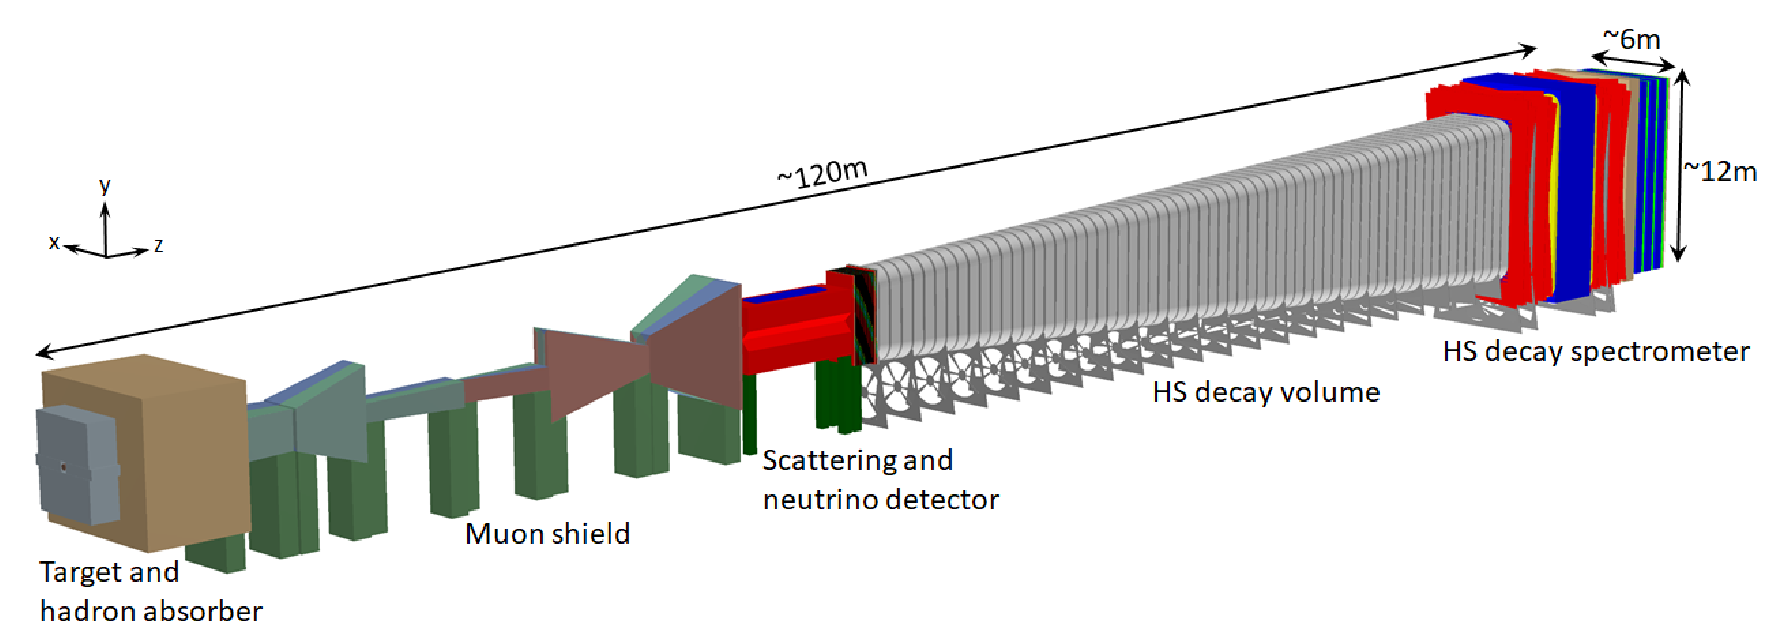
\includegraphics[width=1.\textwidth]{pictures/ship_sketch}
	\caption[Overview of the SHiP experiment.]{Overview of the proposed setup for the SHiP experiment. The target on the left is used as a beam dump for the SPS. Most \ac{sm} particles get absorbed by the hadron absorber directly behind the target. A magnetic muon shield deflects the muon, which will not be absorbed by the hadron absorber, away from the beam line. After the muon shield is a scattering and neutrino detector, and afterward, the \SI{50}{\meter} long decay volume in which non \ac{sm} particles created at the target can decay into \ac{sm} particles. Behind the decay volume, the decay spectrometer is placed. To achieve the zero background goal, the Surround Background Tagger is around the decay volume. \cite{ship_coll}}
	\label{fig:ship_sketch}
\end{figure}

One problem for the measurement is \ac{sm} particles entering the decay volume and getting falsely reconstructed as \ac{hs} events in the spectrometer.
An example of such a background is muons deflected by the muon shield and reflected at the walls of the facility into the decay volume, mimicking the decay products of an \ac{hs} event in the spectrometer.
Therefore it is crucial for the zero background requirement to detect the particles entering the decay volume and tag every event that could be caused by the entering particle as background.
This task is meant to be done by the \ac{sbt}.
As the name suggests, it surrounds the \ac{hs} decay volume, detecting particles entering it.
It is currently in development and this thesis is part of the R\&D effort toward it.
In the following, the \ac{sbt} and the principles of the different parts are described.
The details of the different parts important for this thesis are presented in more detail in the next chapter.

To make the tagging of background events possible and efficient and avoid the incorrect tagging of many \ac{hs} events different pieces of information need to be known about the particles entering the decay volume.
These pieces of information are the energy of the entering particles, the time at which they are entering the decay volume, and the space coordinates at which they are entering.
Therefore the \ac{sbt} is designed as a five-dimensional tagger.
It will consist of approximately 2000 cells that form the walls on the side as well as the top and bottom of the vacuum decay chamber.
The structure is shown in \autoref{fig:sbt}.
In order to fit the overall truncated pyramid shape of the decay volume, the cells have an unsymmetric shape, an example is shown in \autoref{fig:sbt}.
Both of the long edges are parallel, but the shorter sides are not.
The depth of the cells is \SI{20}{\centi\meter} and the wall thickness is planned to be \SI{2}{\centi\meter} \cite{}.
For the detection of particles, a liquid scintillator will be filled into the cells.
A particle passing through one or more cells will deposit energy in the scintillator, causing the emittance of scintillation light.
The amount of emitted light is correlated to the amount of energy deposited in the scintillator.
Two \acp{wom}, PMMA tubes coated with wavelengthshifting paint, are placed in each cell to collect the scintillation light and guide it to an array of \acp{sipm}.
The signals from the \acp{sipm} can be amplified, digitized, and further processed.
Both a \ac{wom} and a \ac{sipm} array are shown in \autoref{fig:sbt}.
\begin{figure}
	\centering
	\begin{subfigure}[b]{0.32\textwidth}
		\centering
		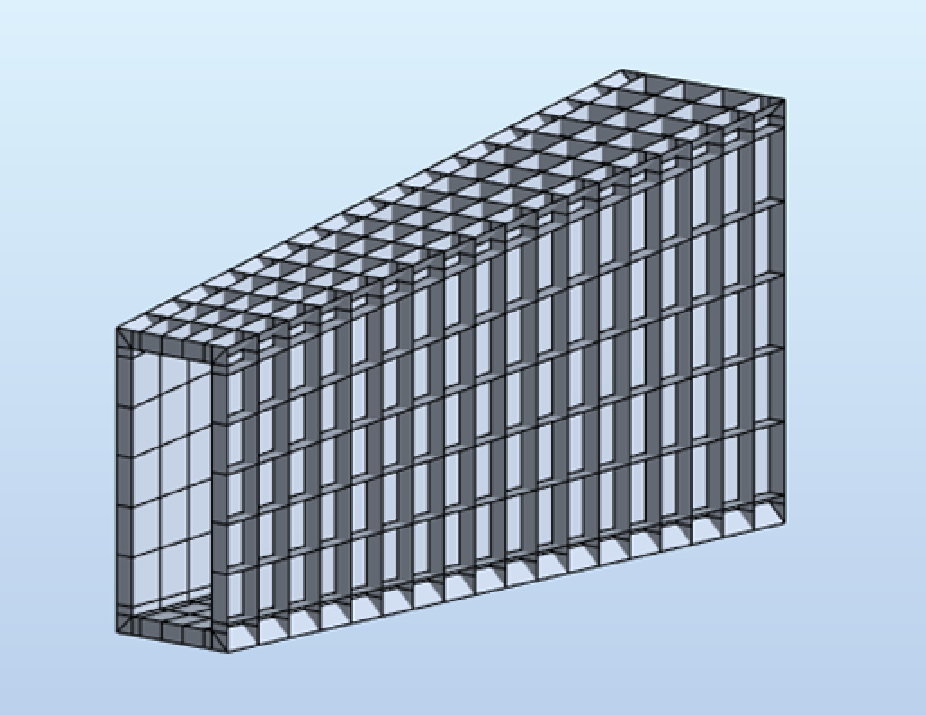
\includegraphics[width=1.\textwidth]{pictures/sbt_structure_sceleton}
		\caption{}
		\label{fig:sbt_structure_sceleton}
	\end{subfigure}
	\begin{subfigure}[b]{0.24\textwidth}
		\centering
		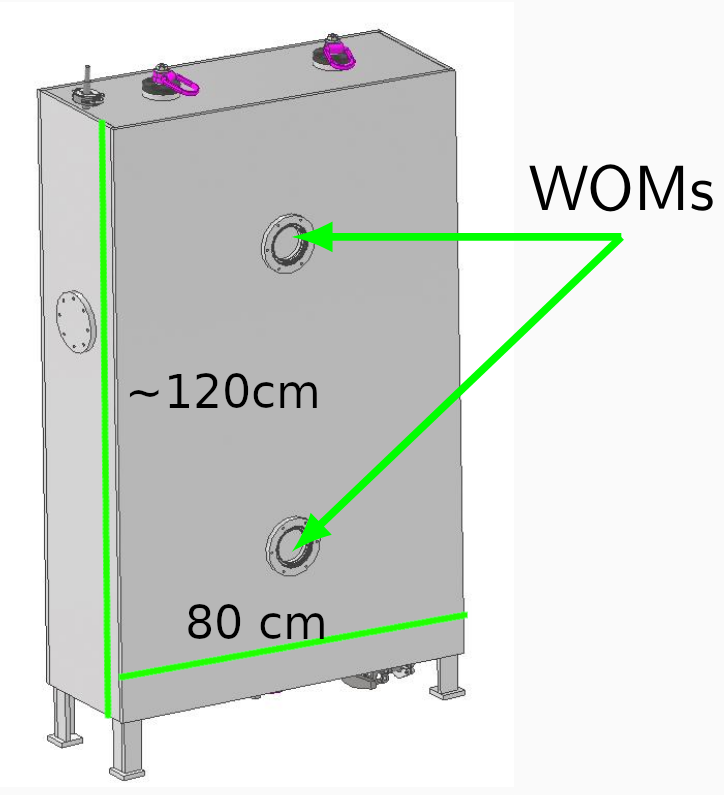
\includegraphics[width=1.\textwidth]{pictures/sbt_structure_cell}
		\caption{}
		\label{fig:sbt_structure_cell}
	\end{subfigure}
	\begin{subfigure}[b]{0.42\textwidth}
		\centering
		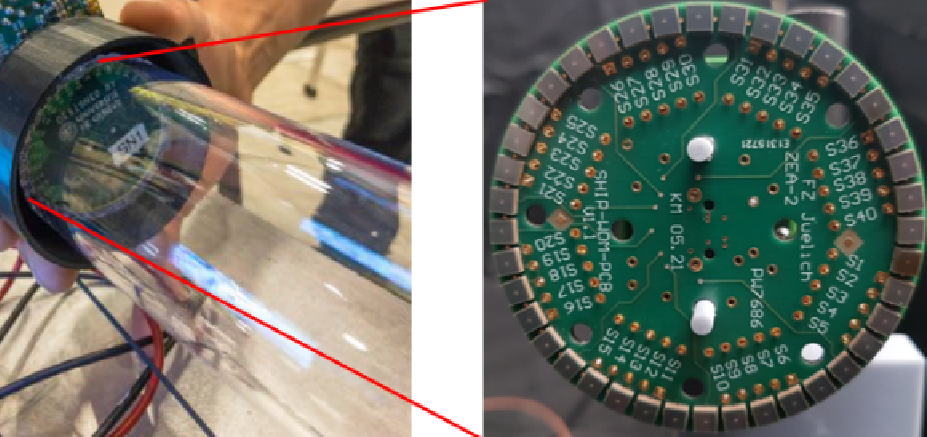
\includegraphics[width=1.\textwidth]{pictures/sbt_structure_wom}
		\caption{}
		\label{fig:sbt_structure}
	\end{subfigure}
	\caption[Overview of the Surrounding Background Tagger]{The structure of the Surrounding Background Tagger (SBT). Left is the SBT with approximately 2000 cells \cite{}. Then the prototype of one example cell is shown in b) \cite{}. The light produced by the liquid scintillator inside the cells is captured by two Wavelengthshifting Optical Modules (WOMs) per cell, an example is shown in c) \cite{}, and then guided to an array of Silicon Photomultiplier which will detect the light.}
 	\label{fig:sbt}
\end{figure}

This thesis is in the scope of the R\&D of the \ac{sbt}.
For the R\&D of the \ac{sbt}, a prototype of one of the cells was built, with which important parts can be tested.
Starting from the cell's material itself, a reflecting coating on the inside of the cell, the coated \acp{wom}, and the \acp{sipm}, to name a few.
This thesis is about the readout of the \acp{wom} of the prototype.
Since the \ac{asic} meant to be used for the readout in the \ac{sbt} is in development by the Forschungszentrum Jülich and not yet finished, another readout is needed for the One Cell Prototype in order to test it.
The next chapter presents the One Cell Prototype with a focus on the \ac{wom} readout.
